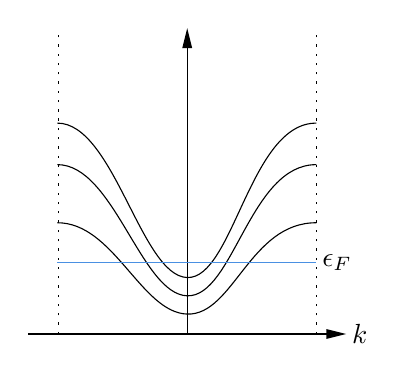
\begin{tikzpicture}[x=0.75pt,y=0.75pt,yscale=-0.8,xscale=0.8]
    %uncomment if require: \path (0,300); %set diagram left start at 0, and has height of 300
    
    %Straight Lines [id:da4138677847824037] 
    \draw    (122,238) -- (311.5,238) ;
    \draw [shift={(313.5,238)}, rotate = 180] [fill={rgb, 255:red, 0; green, 0; blue, 0 }  ][line width=0.08]  [draw opacity=0] (12,-3) -- (0,0) -- (12,3) -- cycle    ;
    %Straight Lines [id:da19072401139926076] 
    \draw    (217.75,238) -- (217.75,55.85) ;
    \draw [shift={(217.75,53.85)}, rotate = 90] [fill={rgb, 255:red, 0; green, 0; blue, 0 }  ][line width=0.08]  [draw opacity=0] (12,-3) -- (0,0) -- (12,3) -- cycle    ;
    %Curve Lines [id:da6883784396806765] 
    \draw    (139.5,171) .. controls (173.5,170.85) and (190,225.15) .. (217.75,226) .. controls (245.5,226.85) and (255.5,170.85) .. (295.5,171) ;
    %Straight Lines [id:da37445061519997136] 
    \draw  [dash pattern={on 0.84pt off 2.51pt}]  (140,238) -- (140,53.85) ;
    %Straight Lines [id:da5423933952599624] 
    \draw  [dash pattern={on 0.84pt off 2.51pt}]  (295.5,238) -- (295.5,53.85) ;
    %Curve Lines [id:da04733929208931942] 
    \draw    (139.5,136) .. controls (173.5,135.85) and (190,214.15) .. (217.75,215) .. controls (245.5,215.85) and (255.5,135.85) .. (295.5,136) ;
    %Curve Lines [id:da41552926054468076] 
    \draw    (139.5,111) .. controls (173.5,110.85) and (190,203.15) .. (217.75,204) .. controls (245.5,204.85) and (255.5,110.85) .. (295.5,111) ;
    %Straight Lines [id:da9886126440781515] 
    \draw [color={rgb, 255:red, 74; green, 144; blue, 226 }  ,draw opacity=1 ]   (139.5,195) -- (295.5,195) ;
    
    % Text Node
    \draw (297.5,195) node [anchor=west] [inner sep=0.75pt]    {$\epsilon _{\text{F}}$};
    % Text Node
    \draw (315.5,238) node [anchor=west] [inner sep=0.75pt]    {$k$};
    
    
    \end{tikzpicture}
    